% ------------------------------------------------------------------------------
% TYPO3 CMS 8.6 - What's New - Chapter "Backend User Interface" (Dutch Version)
%
% @author	Michael Schams <schams.net>
% @license	Creative Commons BY-NC-SA 3.0
% @link		http://typo3.org/download/release-notes/whats-new/
% @language	English
% ------------------------------------------------------------------------------
% LTXE-CHAPTER-UID:		07b25346-95b1df21-a6ebe09a-49f53f41
% LTXE-CHAPTER-NAME:	Backend User Interface
% ------------------------------------------------------------------------------

\section{Gebruikersinterface backend}
\begin{frame}[fragile]
	\frametitle{Gebruikersinterface backend}

	\begin{center}\huge{Hoofdstuk 1:}\end{center}
	\begin{center}\huge{\color{typo3darkgrey}\textbf{Gebruikersinterface backend}}\end{center}

\end{frame}

% ------------------------------------------------------------------------------
% LTXE-SLIDE-START
% LTXE-SLIDE-UID:		85c64141-fa3f855f-5d8162bd-8143f35b
% LTXE-SLIDE-ORIGIN:	4141a9cc-46da51df-9dd87a8b-9b15ac29 English
% LTXE-SLIDE-TITLE:		#12211: Scheduler Page Browser
% LTXE-SLIDE-REFERENCE:	!Feature: #12211 - Usability: Scheduler provide page browser to choose start page
% ------------------------------------------------------------------------------
\begin{frame}[fragile]
	\frametitle{Gebruikersinterface backend}
	\framesubtitle{Taakplanner paginaselector}

	Om de taak voor \textbf{EXT:linkvalidator} te verbeteren is de paginaselector
	toegevoegd om een beginpagina te kiezen.

	\begin{figure}\vspace{-0.2cm}
		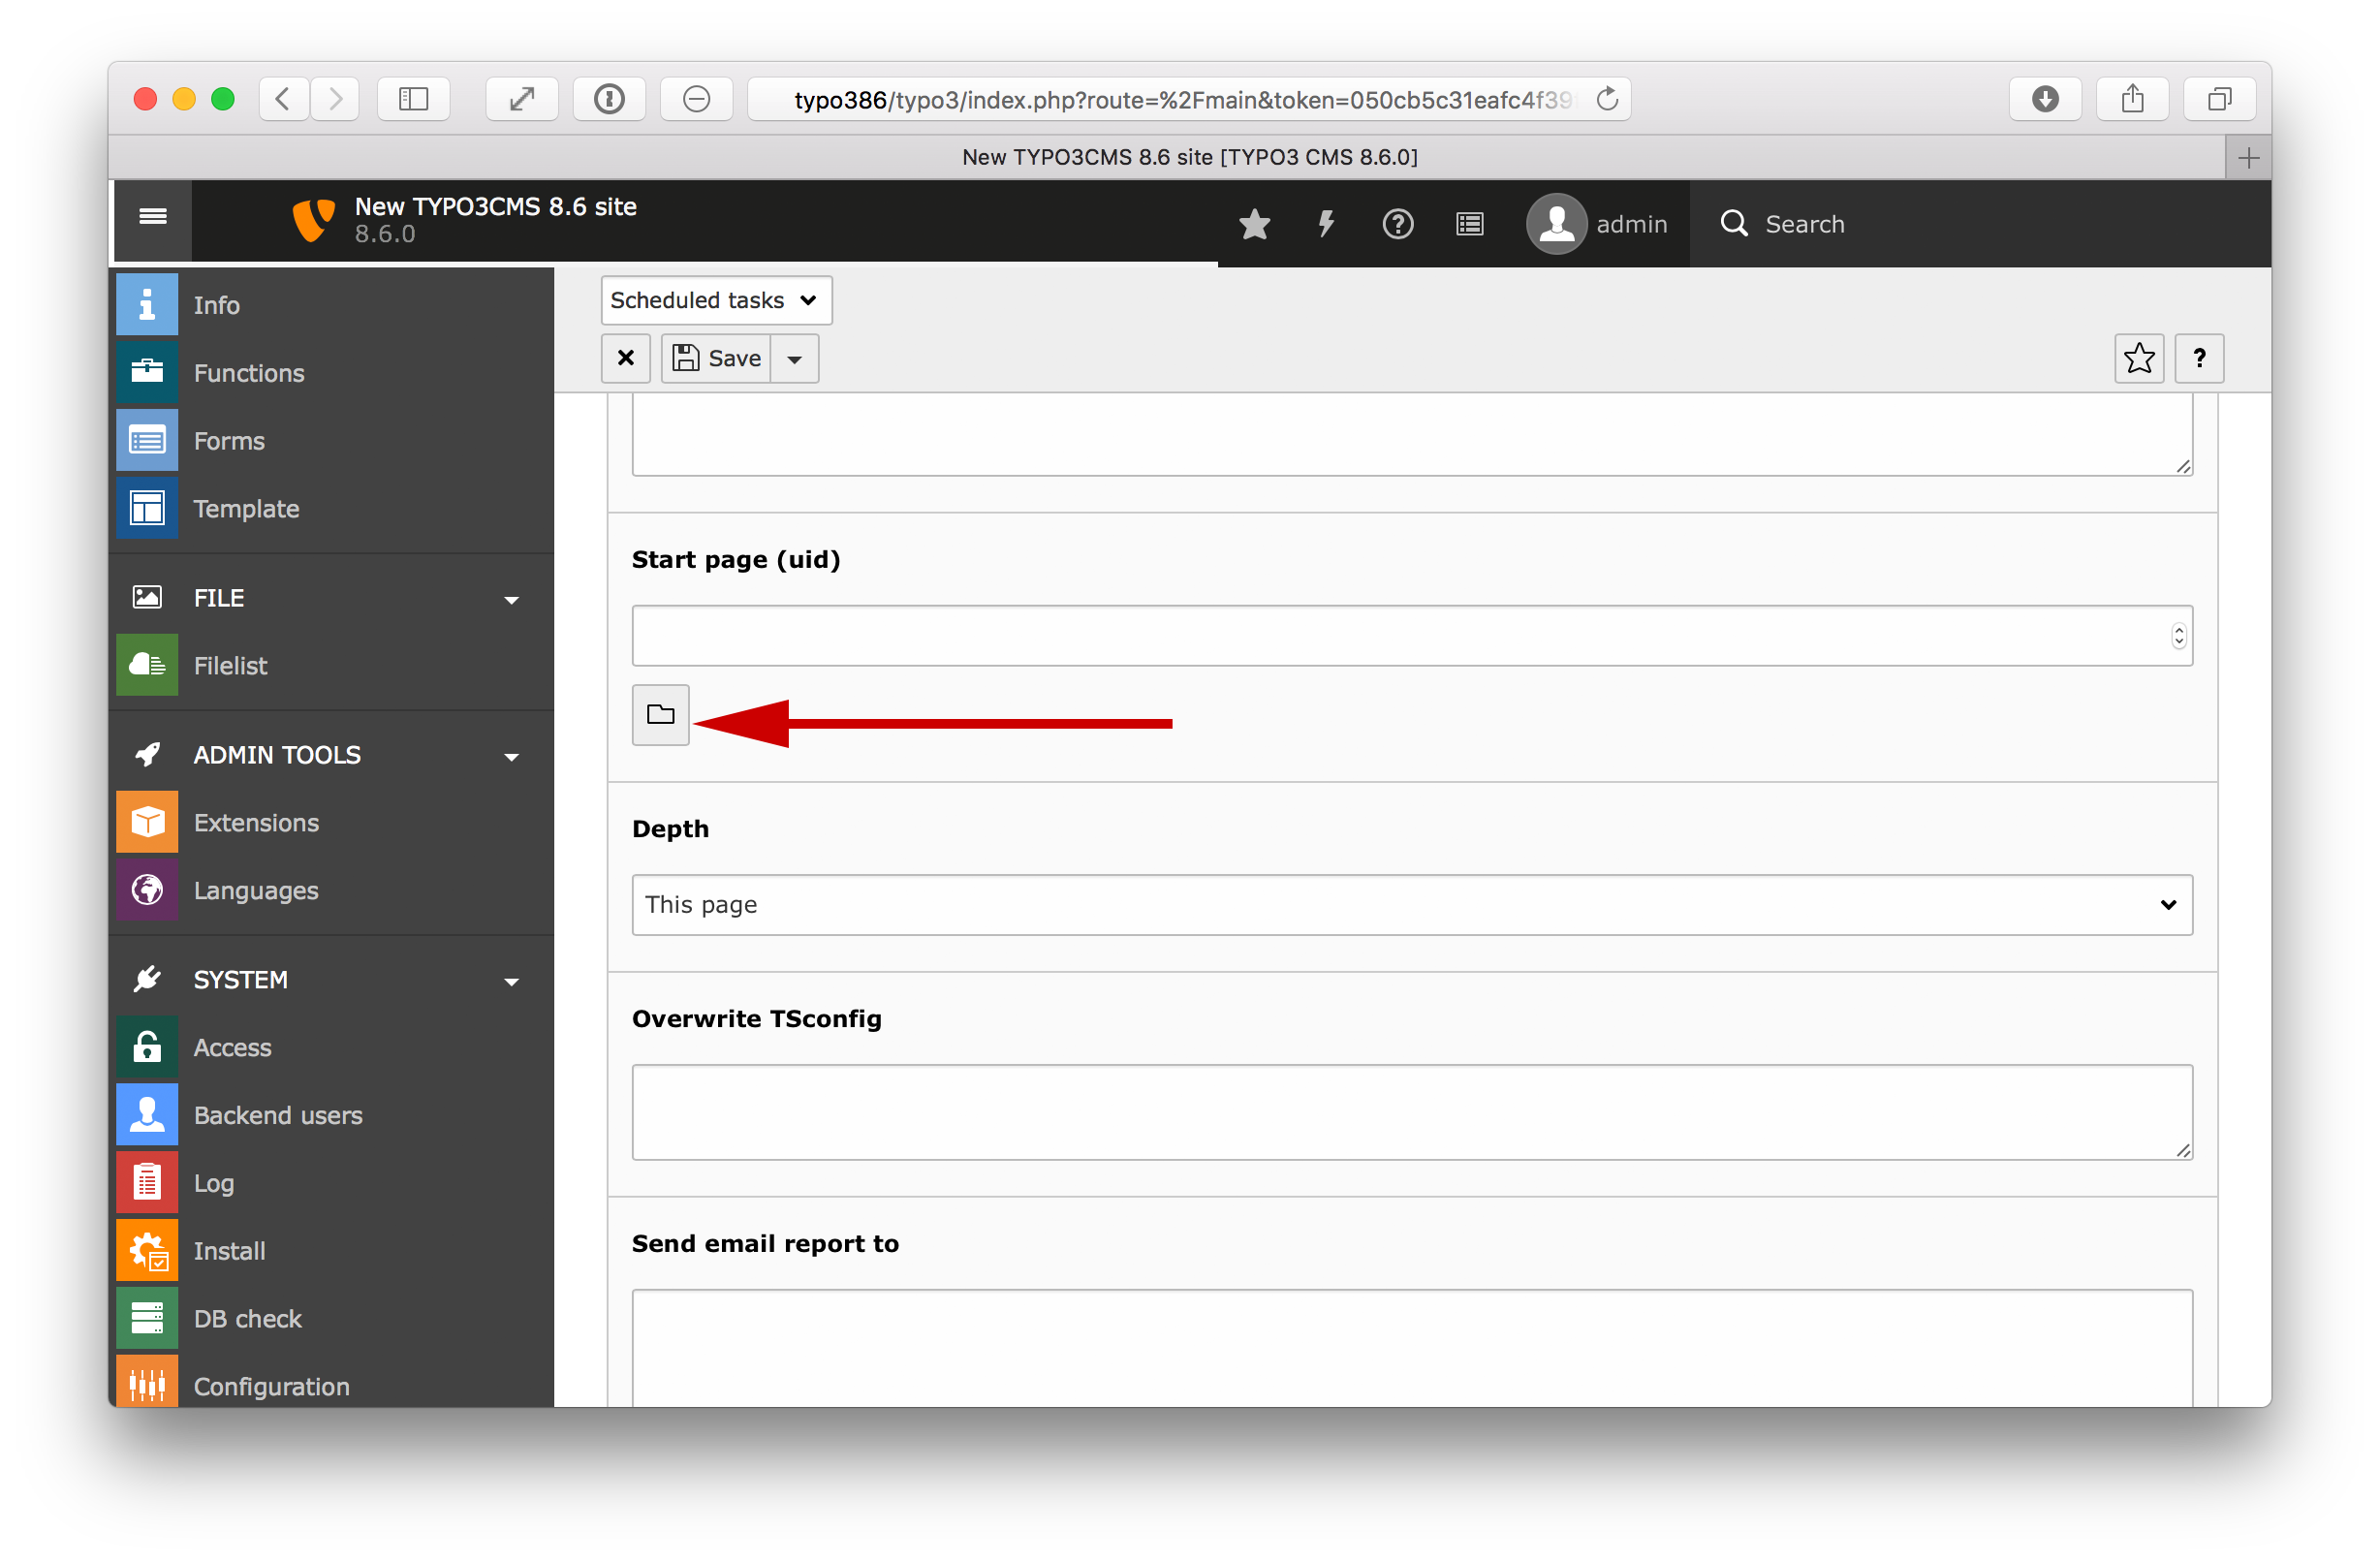
\includegraphics[width=0.67\linewidth]{BackendUserInterface/12211.png}
	\end{figure}

\end{frame}

% ------------------------------------------------------------------------------
% LTXE-SLIDE-START
% LTXE-SLIDE-UID:		5182450b-74d31c93-ceb921b3-5b57c468
% LTXE-SLIDE-ORIGIN:	f924be39-75ae40d9-ba00f0a8-3a6de040 English
% LTXE-SLIDE-TITLE:		#45537: Manually executed tasks
% LTXE-SLIDE-REFERENCE:	!Feature: #45537 - Run manually executed tasks on next cron-run
% ------------------------------------------------------------------------------
\begin{frame}[fragile]
	\frametitle{Gebruikersinterface backend}
	\framesubtitle{Handmatige taken bij de volgende cron uitvoeren}

	\begin{columns}[T]
		\begin{column}{0.3\textwidth}
			Er is een nieuw icoon om aan te geven dat een taak door de cron uitgevoerd moet worden.
			Een nieuwe knop "geselecteerde taken bij de volgende cron job uitvoeren" is ook toegevoegd.
		\end{column}

		\begin{column}{0.7\textwidth}
			\begin{figure}\vspace{-0.6cm}
				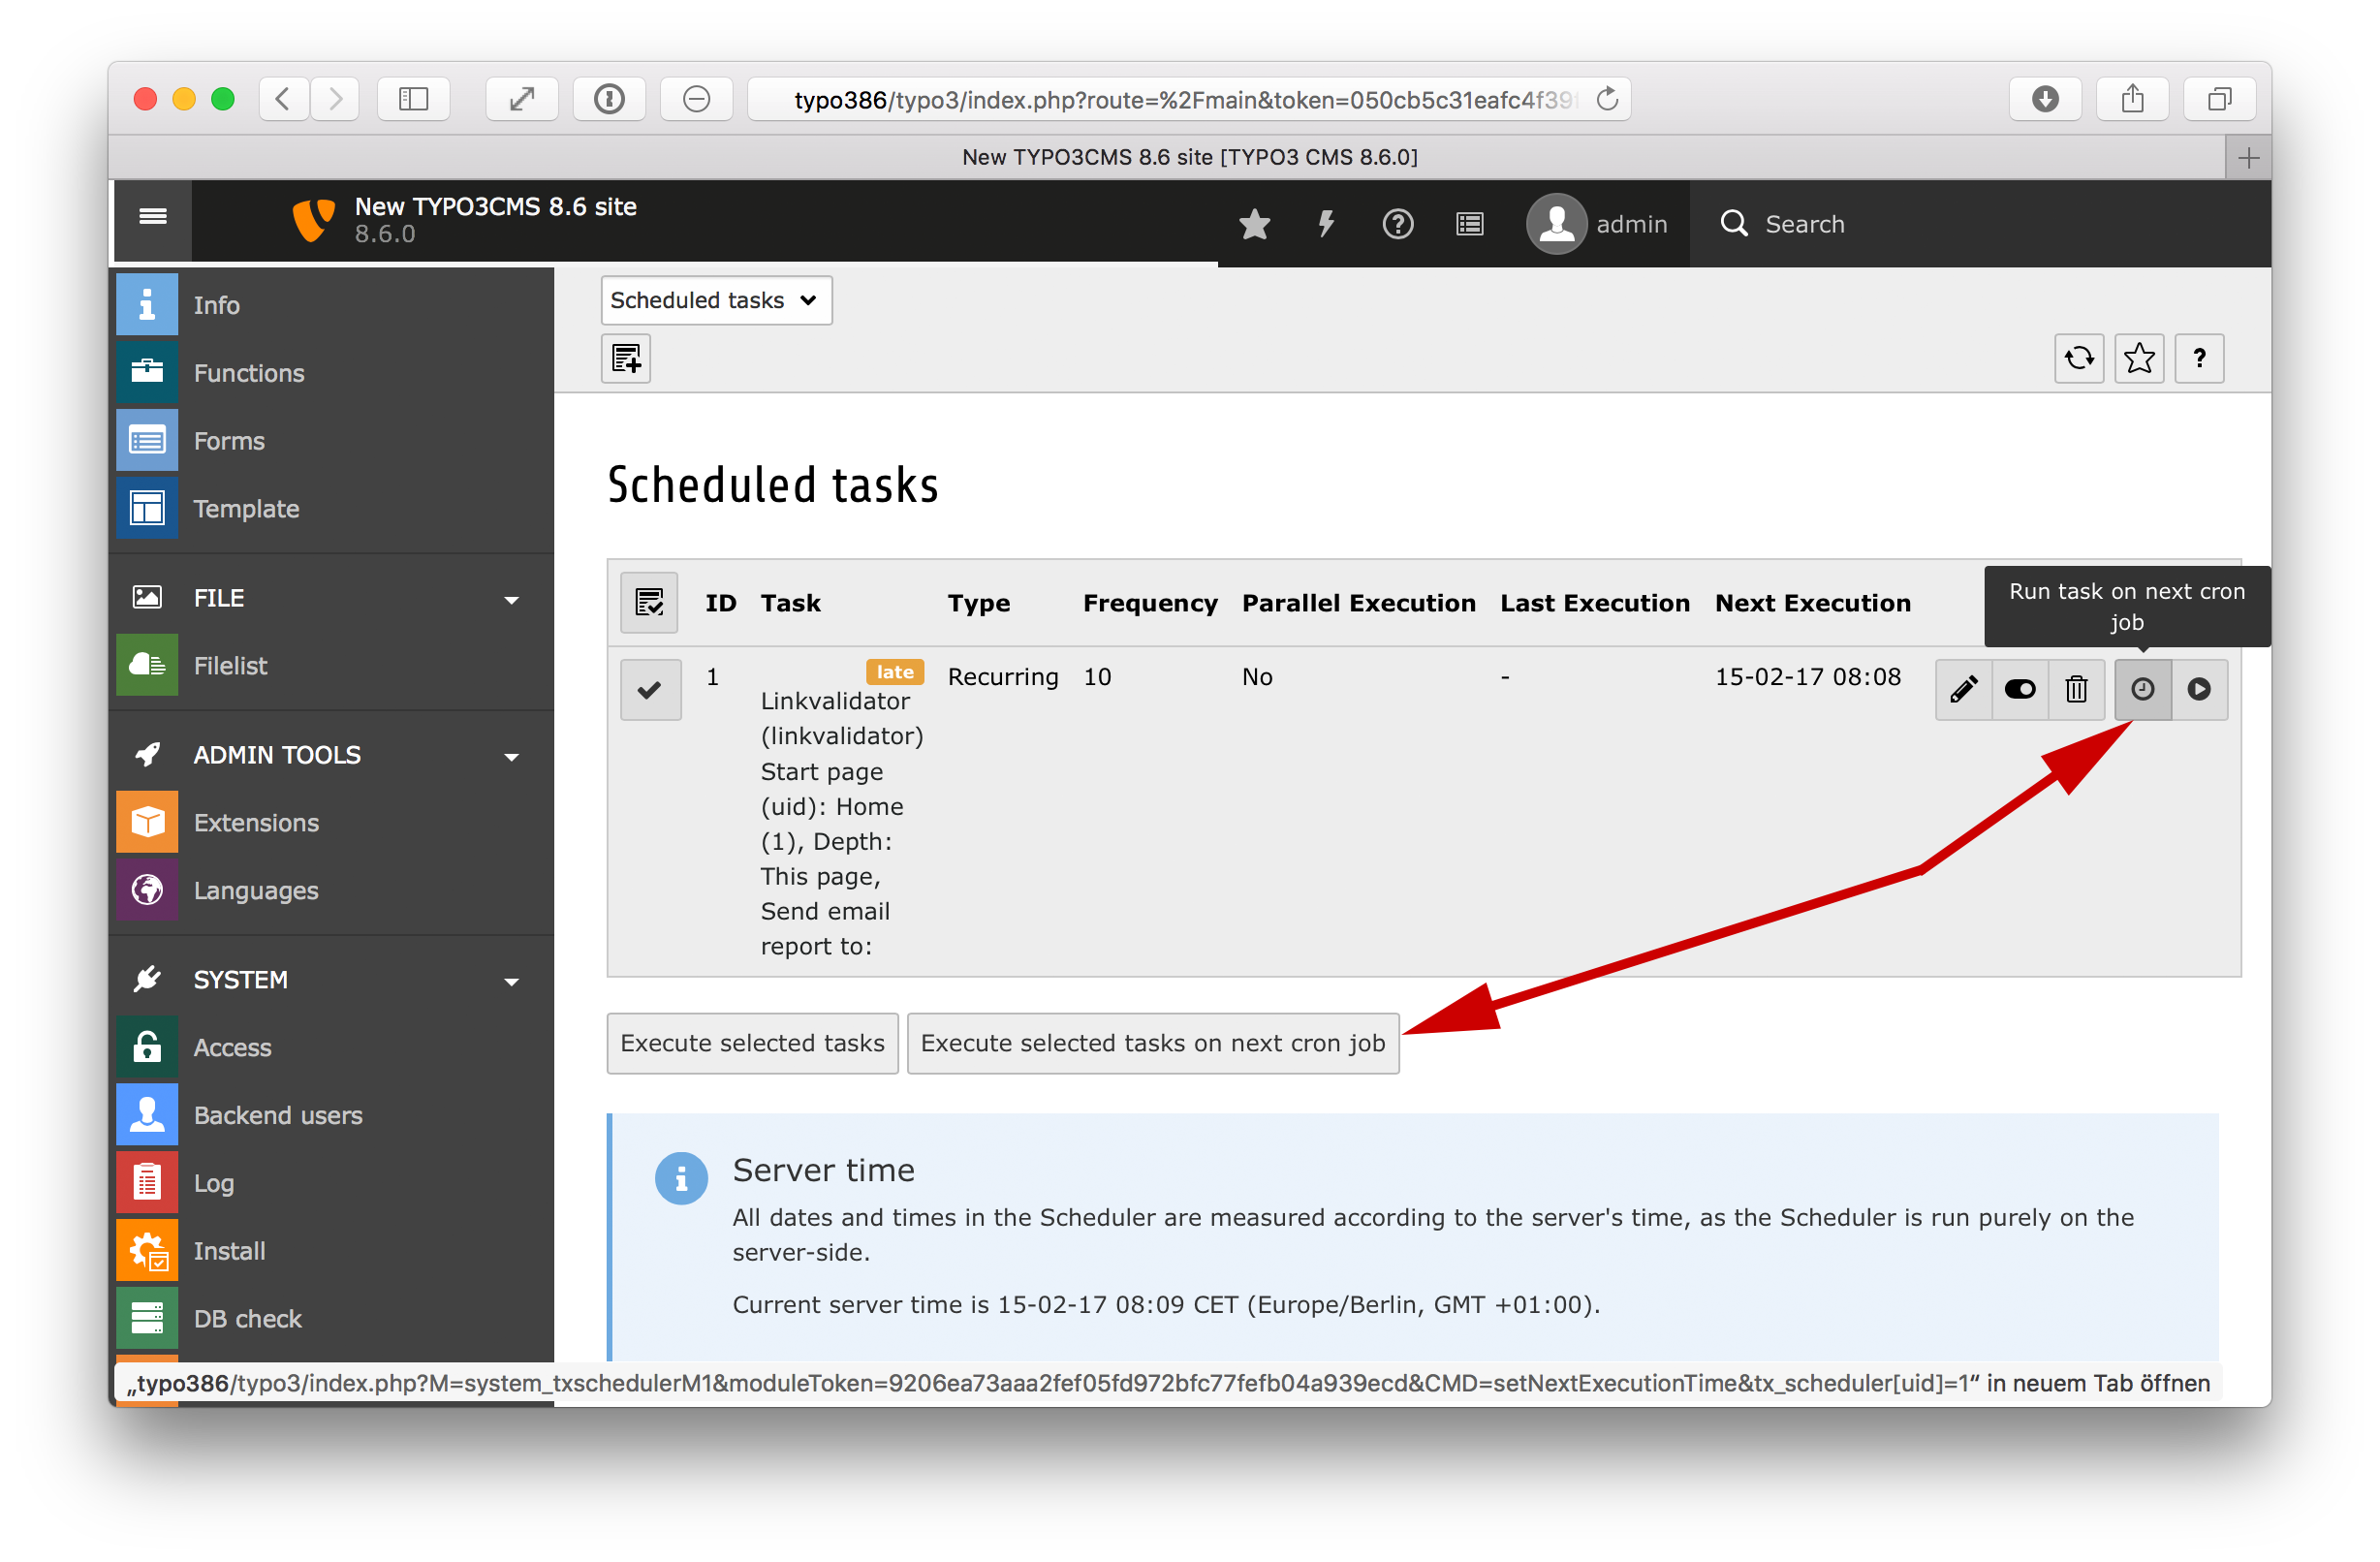
\includegraphics[width=0.99\linewidth]{BackendUserInterface/45537.png}
			\end{figure}
		\end{column}
	\end{columns}

\end{frame}

% ------------------------------------------------------------------------------
% LTXE-SLIDE-START
% LTXE-SLIDE-UID:		5d9eda7f-fe30bf37-95b4780b-b77a7e47
% LTXE-SLIDE-ORIGIN:	b6d6054e-21291d35-479a0095-a6e82a4f English
% LTXE-SLIDE-TITLE:		#47135: Paste Icon and Modal
% LTXE-SLIDE-REFERENCE:	!Feature: #51291 - Synchronized field values in localized records
% ------------------------------------------------------------------------------
\begin{frame}[fragile]
	\frametitle{Gebruikersinterface backend}
	\framesubtitle{Icoon plakken en popup}

	Zodra het normale klembord een item bevat, komt er een enkel icoon voor plakken in de
	pagina-module. Na het klikken op het icoon verschijnt een popup om de actie te bevestigen.

	\begin{figure}\vspace{-0.2cm}
		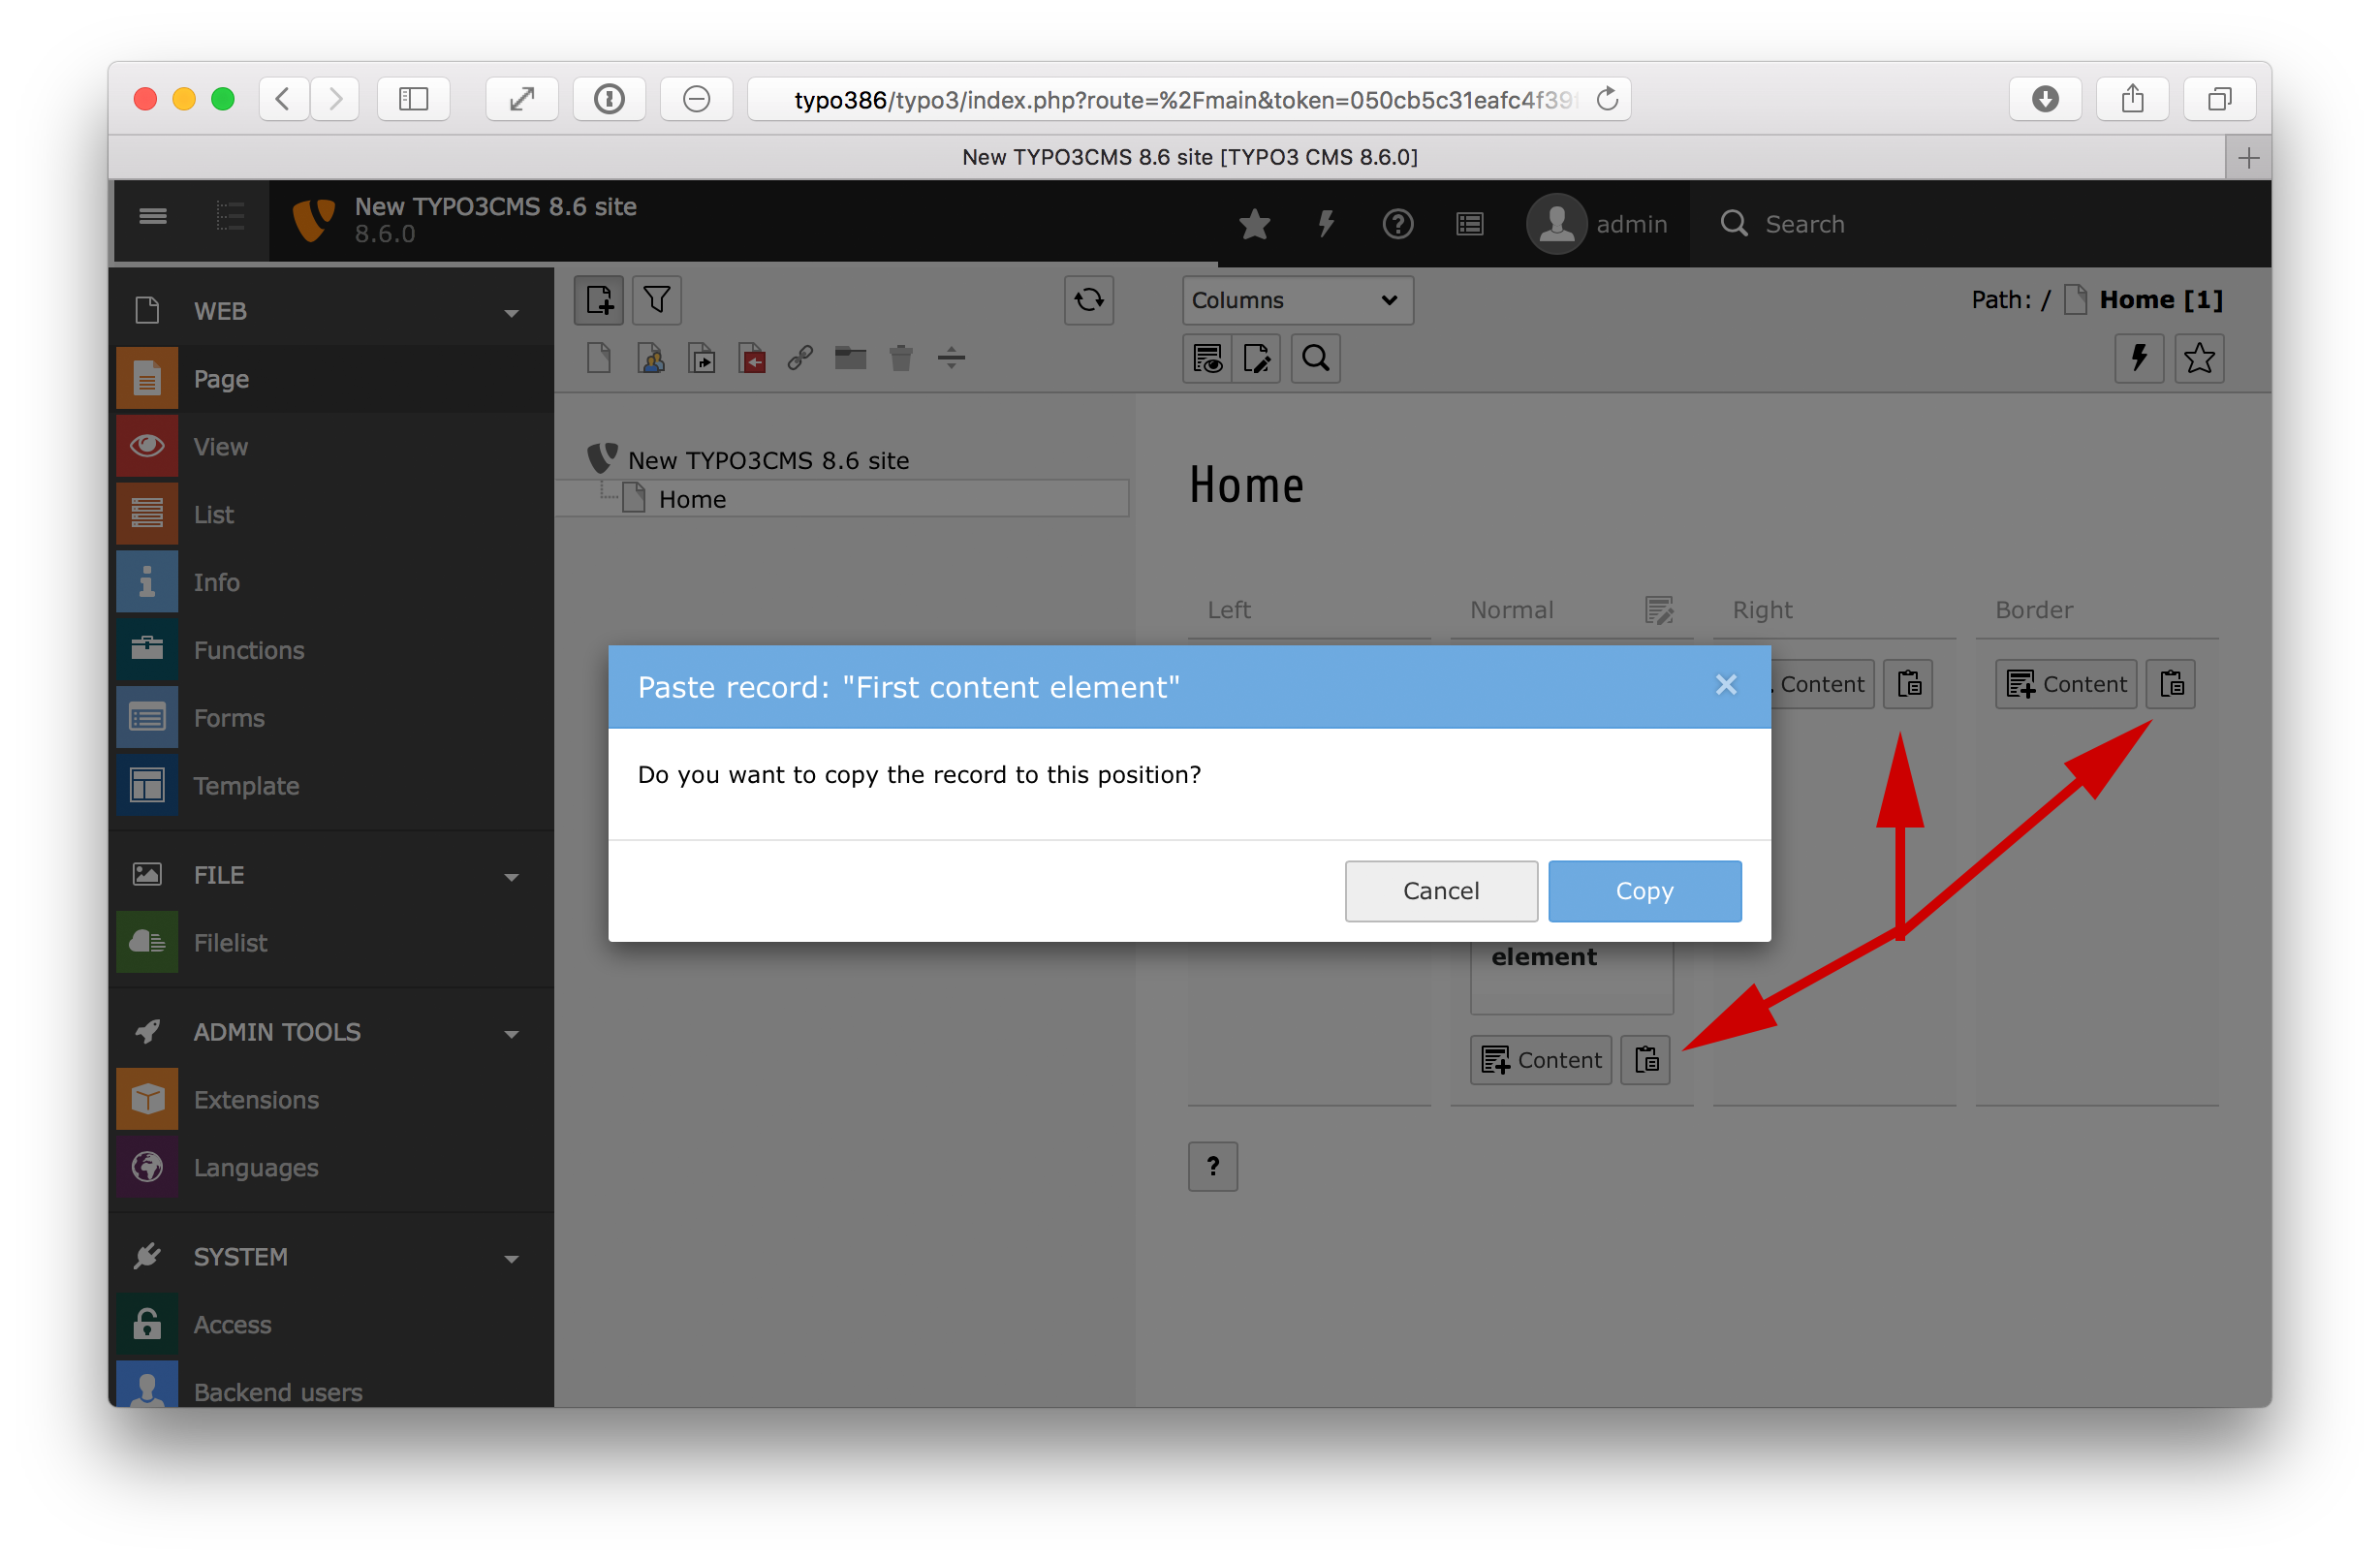
\includegraphics[width=0.63\linewidth]{BackendUserInterface/47135.png}
	\end{figure}

\end{frame}

% ------------------------------------------------------------------------------
% LTXE-SLIDE-START
% LTXE-SLIDE-UID:		4451f4bb-6094dcb5-ace4f24d-31128b0c
% LTXE-SLIDE-ORIGIN:	b31e455f-fce042ed-e3670436-9e72983c English
% LTXE-SLIDE-TITLE:		#67243: Folding of Scheduler Task Groups
% LTXE-SLIDE-REFERENCE:	!Feature: #67243 - Implement folding of scheduler task groups
% ------------------------------------------------------------------------------
\begin{frame}[fragile]
	\frametitle{Gebruikersinterface backend}
	\framesubtitle{Samenvouwen van taakplannergroepen}

	Als taakgroepen worden gebruikt worden de taken in de lijst gegroepeerd afgebeeld.
	Een klik op de regel met de groepstitel verbergt of toont nu de taken in de groep.

	\begin{figure}\vspace{-0.3cm}
		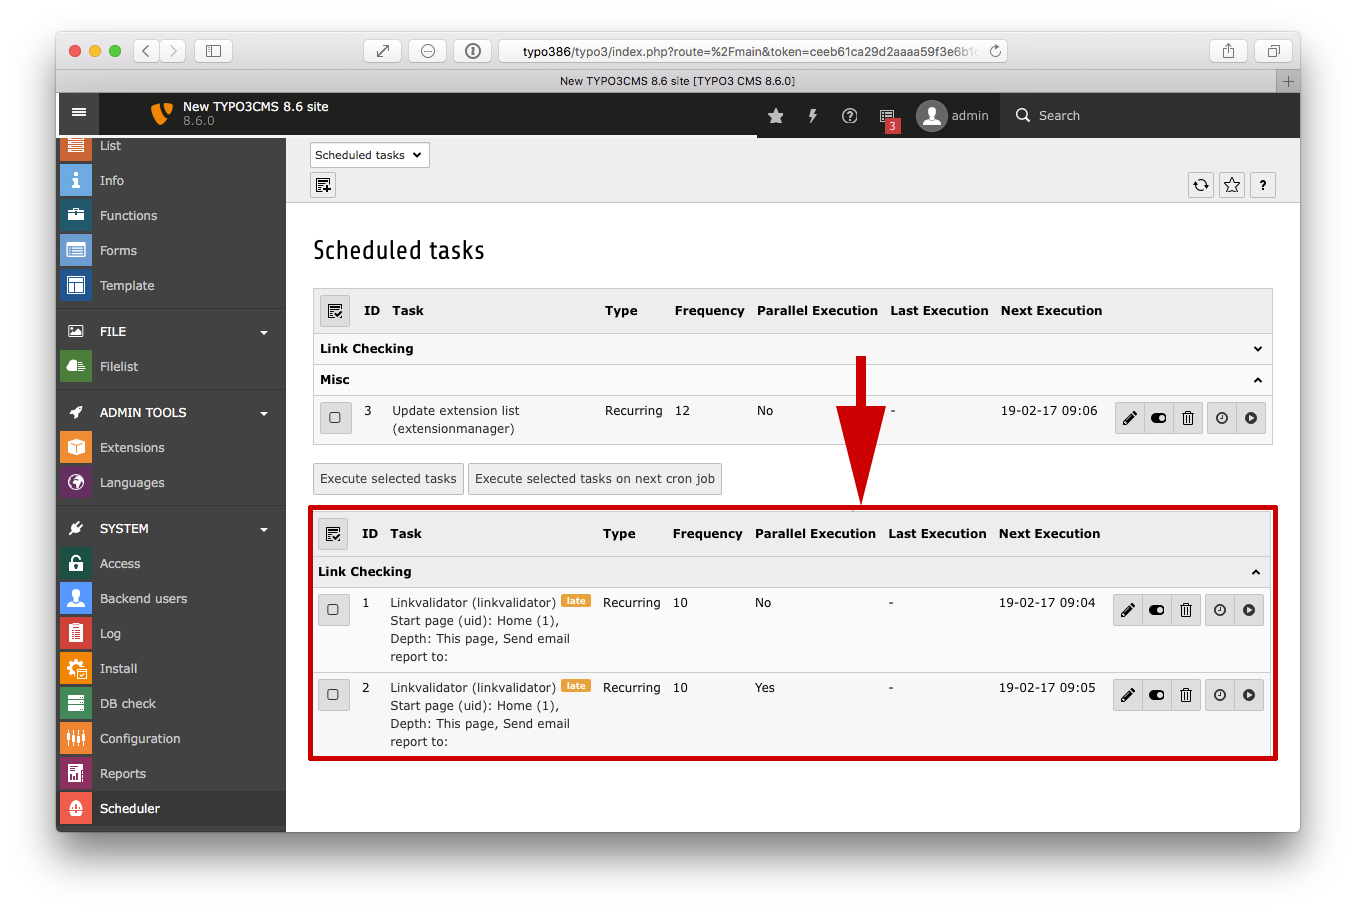
\includegraphics[width=0.60\linewidth]{BackendUserInterface/67243.png}
	\end{figure}

\end{frame}

% ------------------------------------------------------------------------------
% LTXE-SLIDE-START
% LTXE-SLIDE-UID:		d8d515d6-c3a4c0c9-4ceb416d-b69435ae
% LTXE-SLIDE-ORIGIN:	14fe5a0b-2a22a6ce-325b5de1-ef26ce50 English
% LTXE-SLIDE-TITLE:		#69572: Page Module Notice
% LTXE-SLIDE-REFERENCE:	!Feature: #69572 - Page module Notice "Content is also shown on:"
% ------------------------------------------------------------------------------
\begin{frame}[fragile]
	\frametitle{Gebruikersinterface backend}
	\framesubtitle{Bericht in paginamodule "Inhoud wordt ook getoond op"}

	\begin{columns}[T]
		\begin{column}{.3\textwidth}
			Als paginainhoud wordt geërfd van een andere pagina via "Toon inhoud van pagina"
			dan wordt een melding getoond op de pagina die de inhoud binnenhaalt.
		\end{column}

		\begin{column}{.7\textwidth}
			\begin{figure}\vspace*{-0.6cm}
				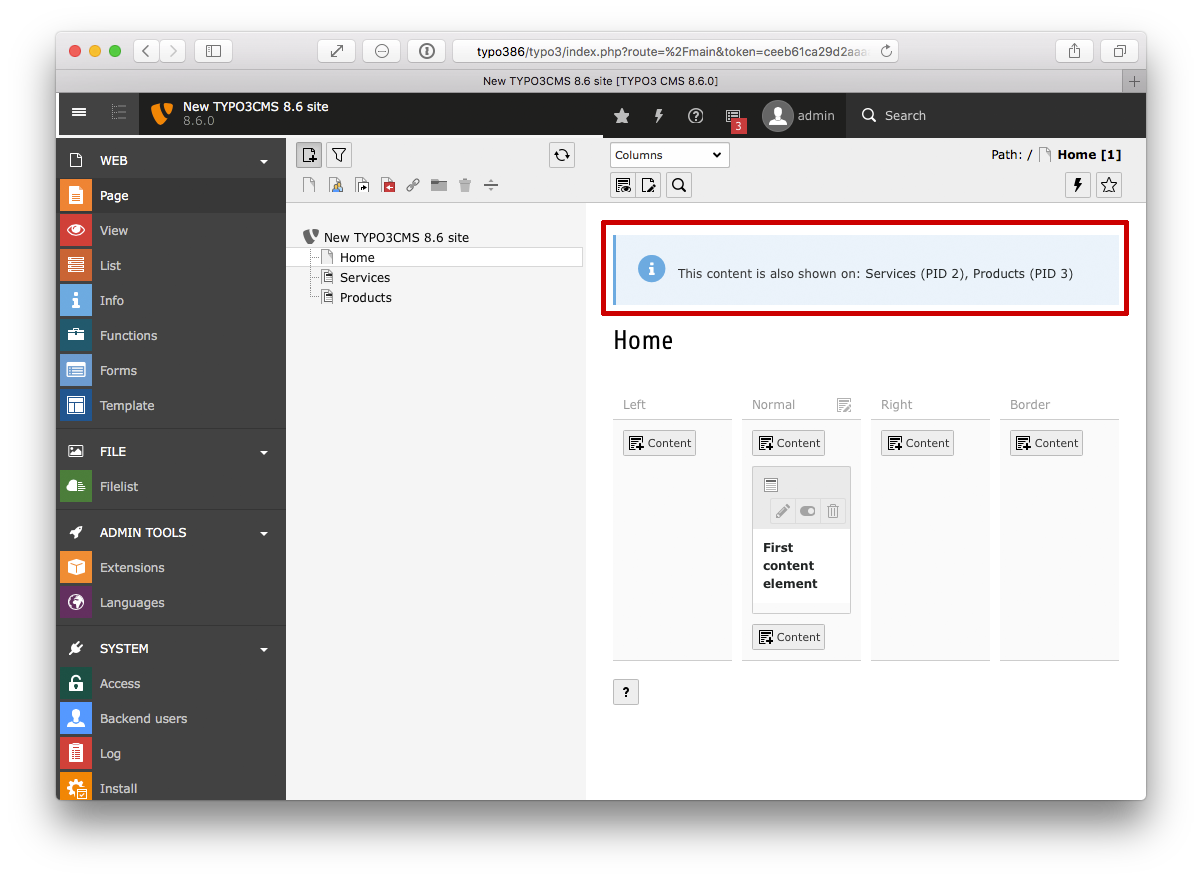
\includegraphics[width=\linewidth]{BackendUserInterface/69572.png}
			\end{figure}
		\end{column}
	\end{columns}

\end{frame}

% ------------------------------------------------------------------------------
% LTXE-SLIDE-START
% LTXE-SLIDE-UID:		00900dd3-31e24a95-faaf7a1f-9584e14d
% LTXE-SLIDE-ORIGIN:	23a4baef-462e7d0c-c8cd4cfc-9dac1f99 English
% LTXE-SLIDE-TITLE:		#75880: Image Manipulation - Multiple Cropping Variants
% LTXE-SLIDE-REFERENCE:	!Feature: #75880 - Implement multiple cropping variants in image manipulation tool
% ------------------------------------------------------------------------------
\begin{frame}[fragile]
	\frametitle{Gebruikersinterface backend}
	\framesubtitle{Grafische bewerkingen - meerdere cropvarianten}

	De tool voor het bewerken van afbeeldingen kan nu meerdere cropvarianten aan (indien geconfigureerd).
	Gebruikers kunnen ook een focusgebied aangeven die altijd binnen het cropgebied valt en het gebied kiezen
	dat altijd zichtbaar moet zijn in het plaatje om de mening te behouden.% -- pas op tekstverloop, het gaat door in de kolom

	\begin{columns}[T]
		\begin{column}{.35\textwidth}
			Om redacteuren een hint te geven welk gebied gebruikt word door andere DOMelementen zoals
			koppen, kunnen meerdere bedekte gebieden gedefinieerd worden.
		\end{column}

		\begin{column}{.65\textwidth}
			\begin{figure}\vspace*{-0.6cm}
				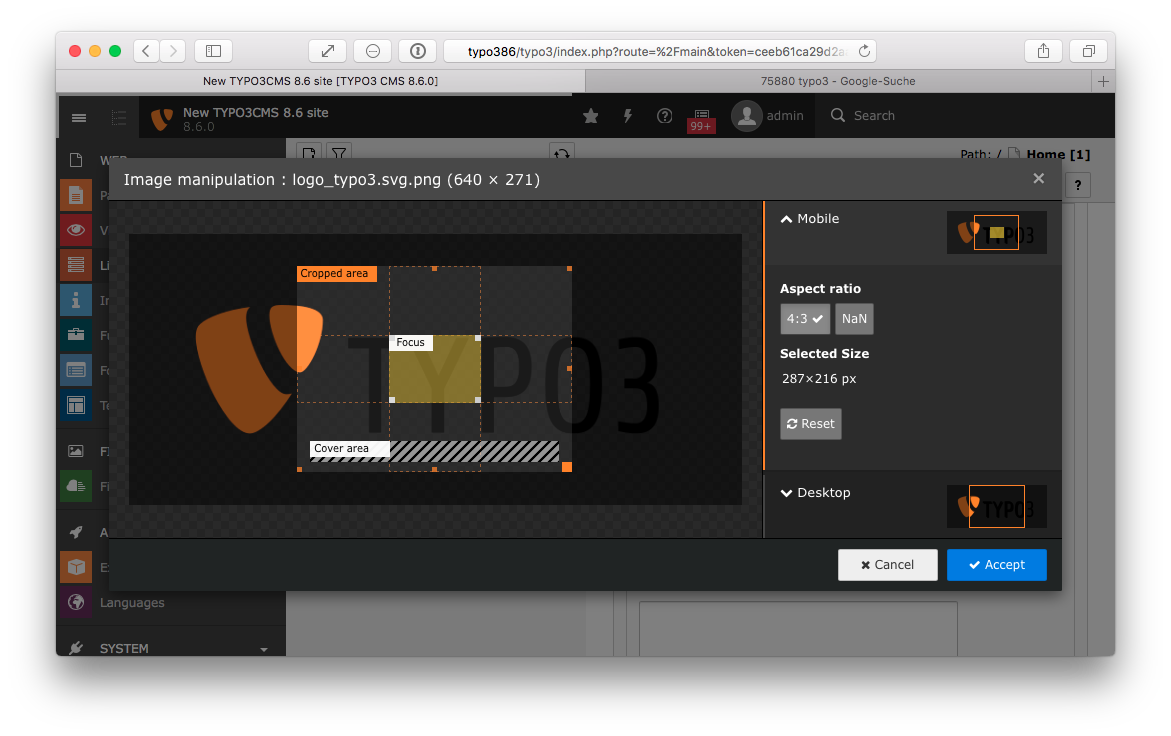
\includegraphics[width=0.99\linewidth]{BackendUserInterface/75880.png}
			\end{figure}
		\end{column}
	\end{columns}

\end{frame}

% ------------------------------------------------------------------------------
% LTXE-SLIDE-START
% LTXE-SLIDE-UID:		cf4cd8a3-130446e0-c6165dc4-edfd517e
% LTXE-SLIDE-ORIGIN:	8f2f695d-f5c6a8bf-5700cf34-d6389ce8 English
% LTXE-SLIDE-TITLE:		#79235: Delete Similar Errors (sys_log)
% LTXE-SLIDE-REFERENCE:	!Feature: #79235 - Add button to delete similar errors from sys_log
% ------------------------------------------------------------------------------
\begin{frame}[fragile]
	\frametitle{Gebruikersinterface backend}
	\framesubtitle{Verwijder gelijksoortige fouten ui \texttt{sys\_log}}

	De log-module van TYPO3 heeft nu een knop om meerdere fouten tegelijk te verwijderen gebaseerd
	op het veld \texttt{details} van de tabel \texttt{sys\_log}. Dit is handig als een fout
	hersteld is waarmee de log volliep.

	\begin{figure}\vspace{-0.2cm}
		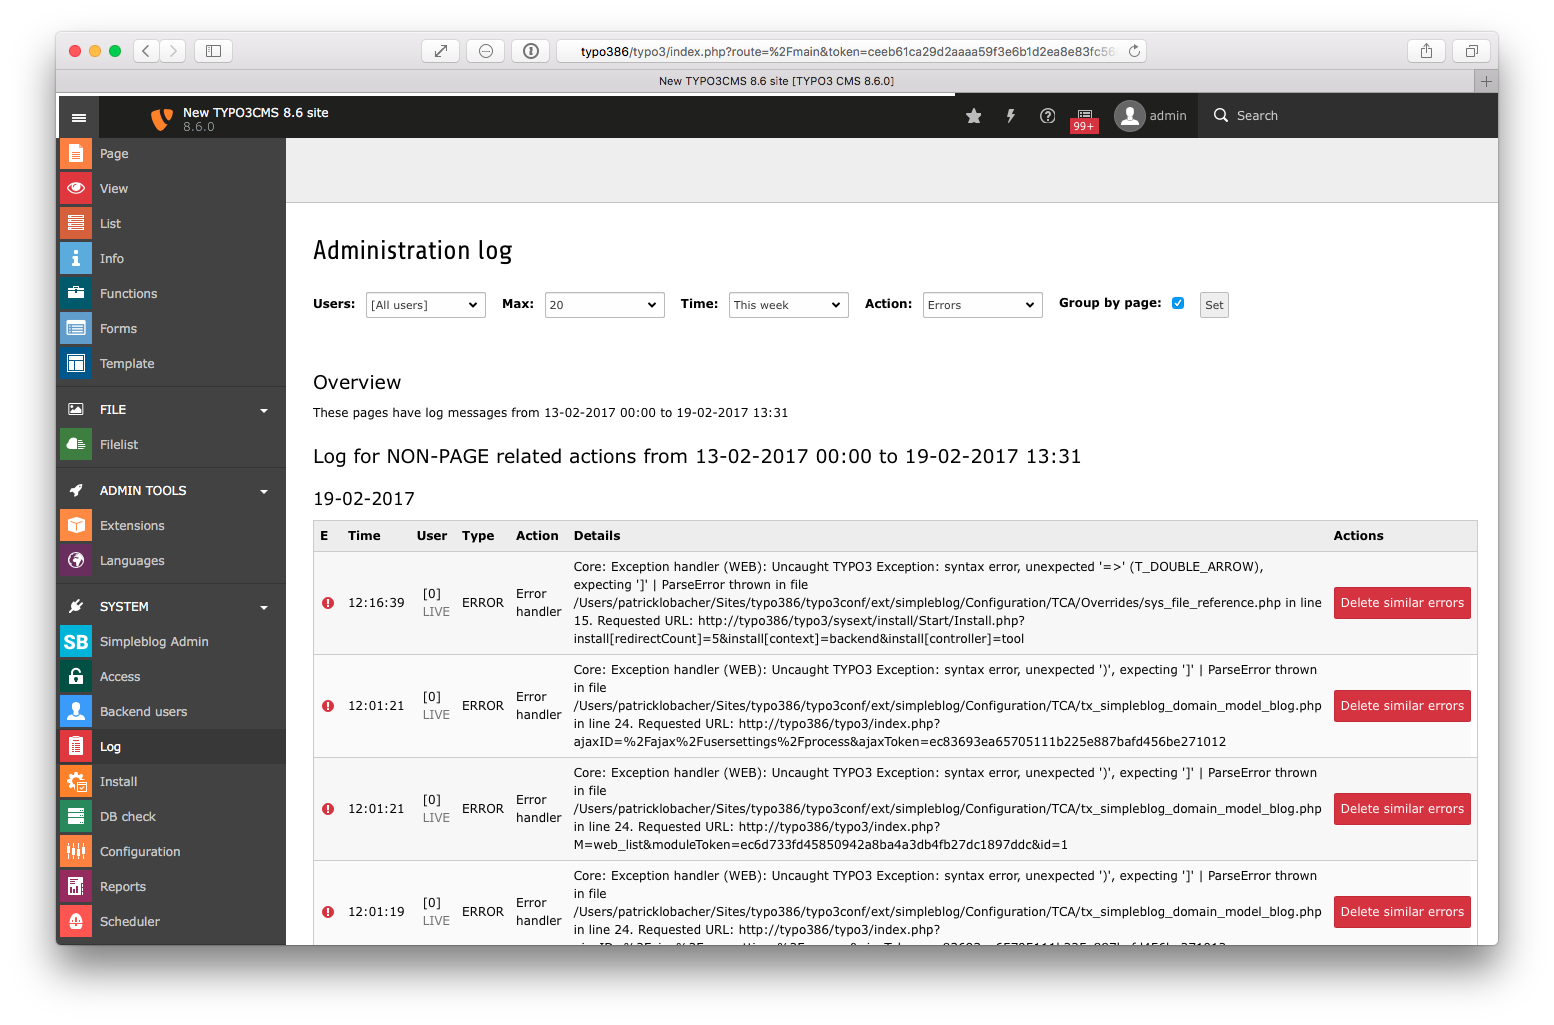
\includegraphics[width=0.60\linewidth]{BackendUserInterface/79235.png}
	\end{figure}

\end{frame}

% ------------------------------------------------------------------------------
% LTXE-SLIDE-START
% LTXE-SLIDE-UID:		7a779cfc-b994bd28-bbb0e335-4d1d3e5e
% LTXE-SLIDE-ORIGIN:	fc878ad9-7b163d51-e579b8b3-9cbe41d9 English
% LTXE-SLIDE-TITLE:		#79467: Form settings button
% LTXE-SLIDE-REFERENCE:	!Feature: #79467 - EXT:form - add form settings button to module header
% ------------------------------------------------------------------------------
\begin{frame}[fragile]
	\frametitle{Gebruikersinterface backend}
	\framesubtitle{\texttt{EXT:form}: knop formulierinstellingen in kop van module}

	Een nieuwe button is toegevoegd aan de modulekop van de formuliereditor.
	De knop activeert een overzicht van formulierinstellingen.

	\begin{figure}\vspace{-0.2cm}
		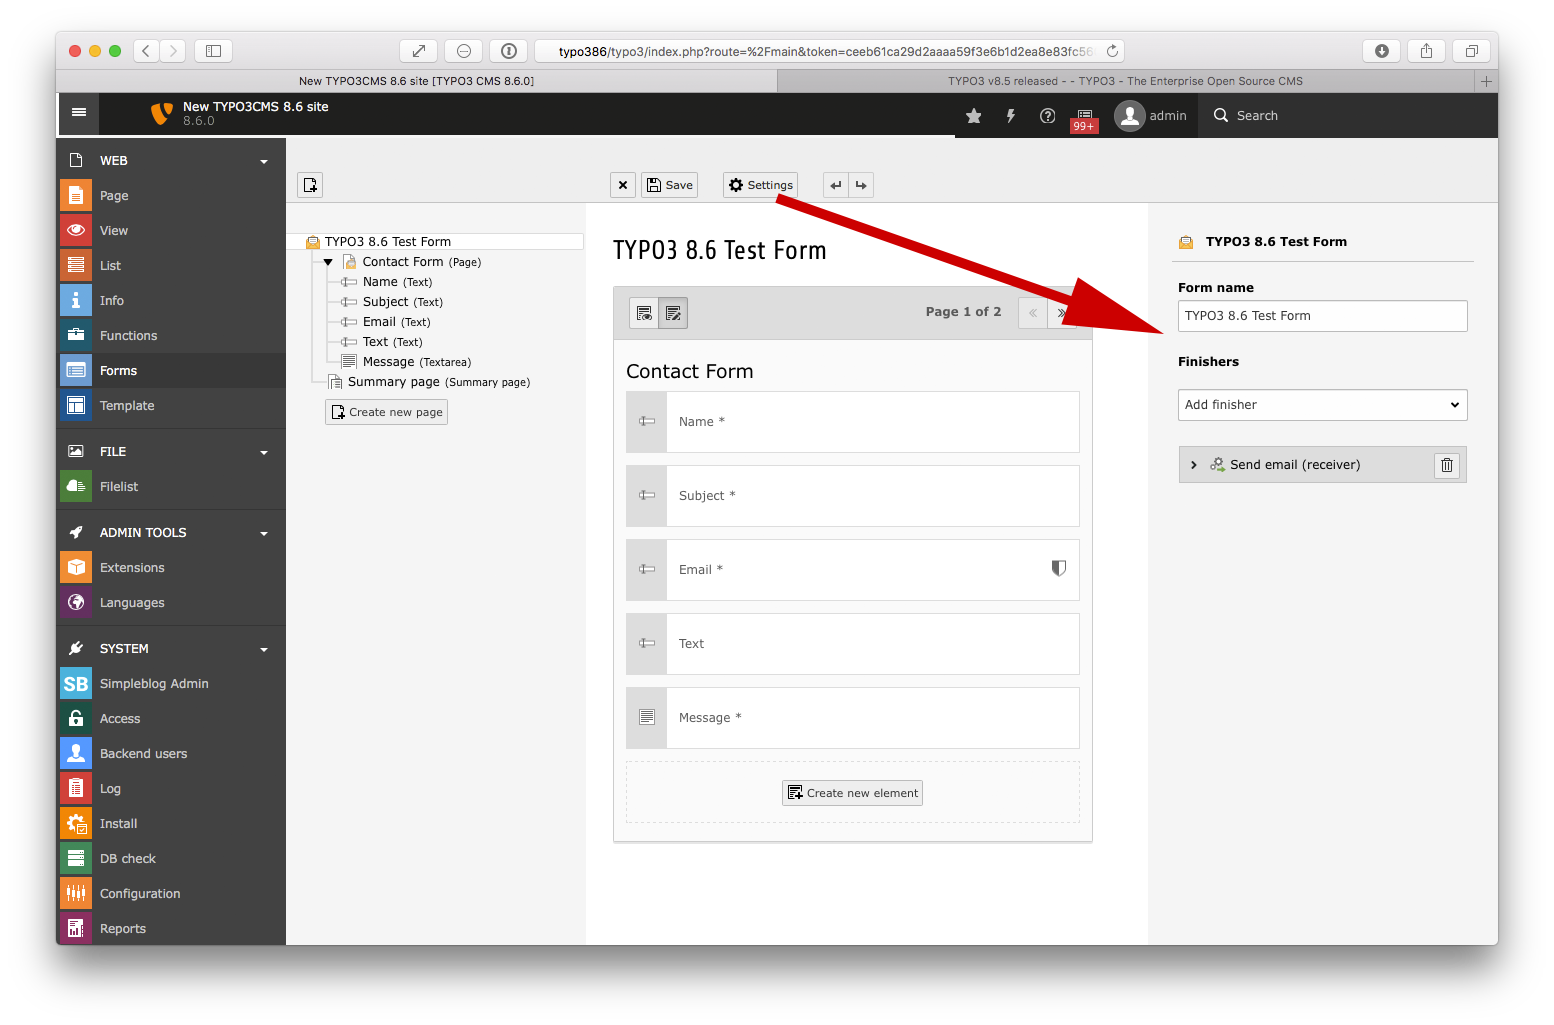
\includegraphics[width=0.675\linewidth]{BackendUserInterface/79467.png}
	\end{figure}

\end{frame}

% ------------------------------------------------------------------------------
% LTXE-SLIDE-START
% LTXE-SLIDE-UID:		e2f314ec-7633adf5-521ef45b-7a1e2eea
% LTXE-SLIDE-ORIGIN:	e1759d2e-8cc138ca-40ce6a34-65354b0e English
% LTXE-SLIDE-TITLE:		#79531: EXT:form - Add multiselect inspector editor
% LTXE-SLIDE-REFERENCE:	!Feature: #79531 - EXT:form - Add multiselect inspector editor
% ------------------------------------------------------------------------------
\begin{frame}[fragile]
	\frametitle{Gebruikersinterface backend}
	\framesubtitle{{EXT:form}: Multi-keuze inspectie-editor}

	\begin{columns}[T]
		\begin{column}{0.35\textwidth}
			Een nieuwe inspectie- editor (d.w.z. een nieuw veldtype), is toegevoegd. Bij
			gebruik kunnen multi- keuzevelden toegevoegd worden aan de inspector.
			Met een multi-keuzeveld kunnen meerdere meta-eigenschappen voor een veld
			ingesteld worden en opgeslagen worden in het ingestelde pad.
		\end{column}

		\begin{column}{0.65\textwidth}
			\begin{figure}\vspace*{-0.6cm}
				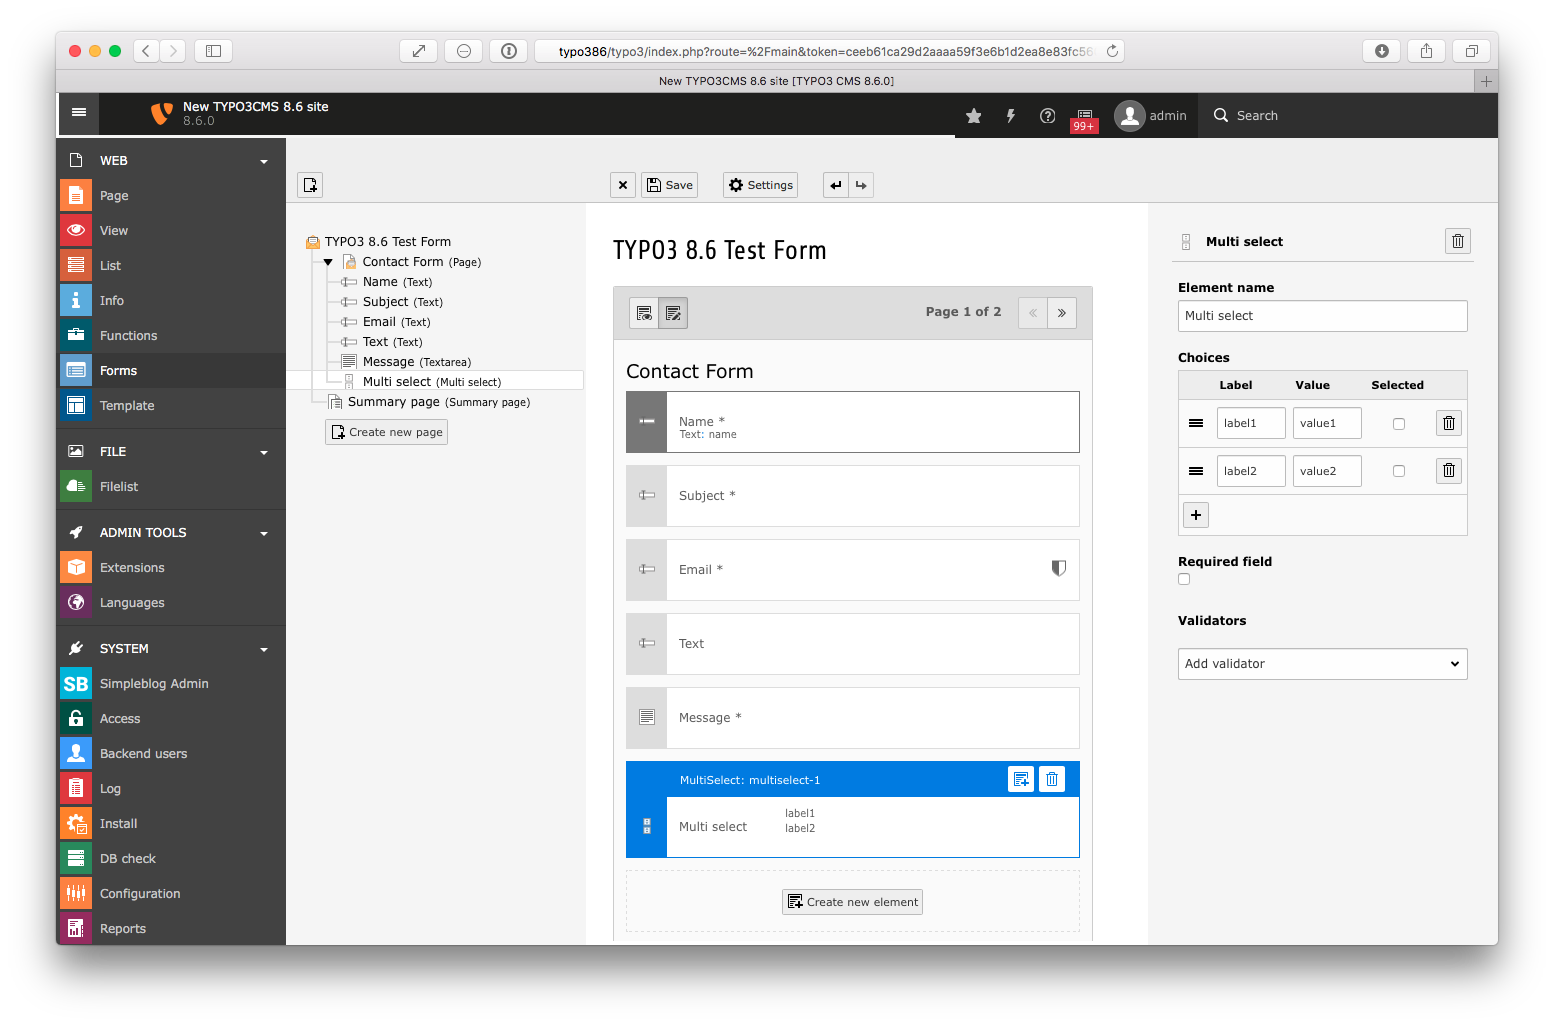
\includegraphics[width=0.99\linewidth]{BackendUserInterface/79531.png}
			\end{figure}
		\end{column}
	\end{columns}

\end{frame}

% ------------------------------------------------------------------------------
% LTXE-SLIDE-START
% LTXE-SLIDE-UID:		c1b4f852-354cdb38-8d02a772-a5a80bdf
% LTXE-SLIDE-ORIGIN:	f6756002-b9aac45f-9460b472-1da819b5 English
% LTXE-SLIDE-TITLE:		#79521: Show list of failed input elements in FormEngine
% LTXE-SLIDE-REFERENCE:	!Feature: #79521 - Show list of failed input elements in FormEngine
% ------------------------------------------------------------------------------
\begin{frame}[fragile]
	\frametitle{Gebruikersinterface backend}
	\framesubtitle{Lijst van fouten in FormEngine}

	\begin{columns}[T]
		\begin{column}{.35\textwidth}
			Als het valideren van invoervelden in de FormEngine niet slaagt wordt nu een knop
			getoond in de knoppen- balk. Deze knop geeft een lijst met de invoervelden die niet
			valideren. Door te klikken op een veld in de lijst krijgt het veld in het formulier
			automatisch de focus.
		\end{column}

		\begin{column}{.65\textwidth}
			\begin{figure}\vspace*{-0.6cm}
				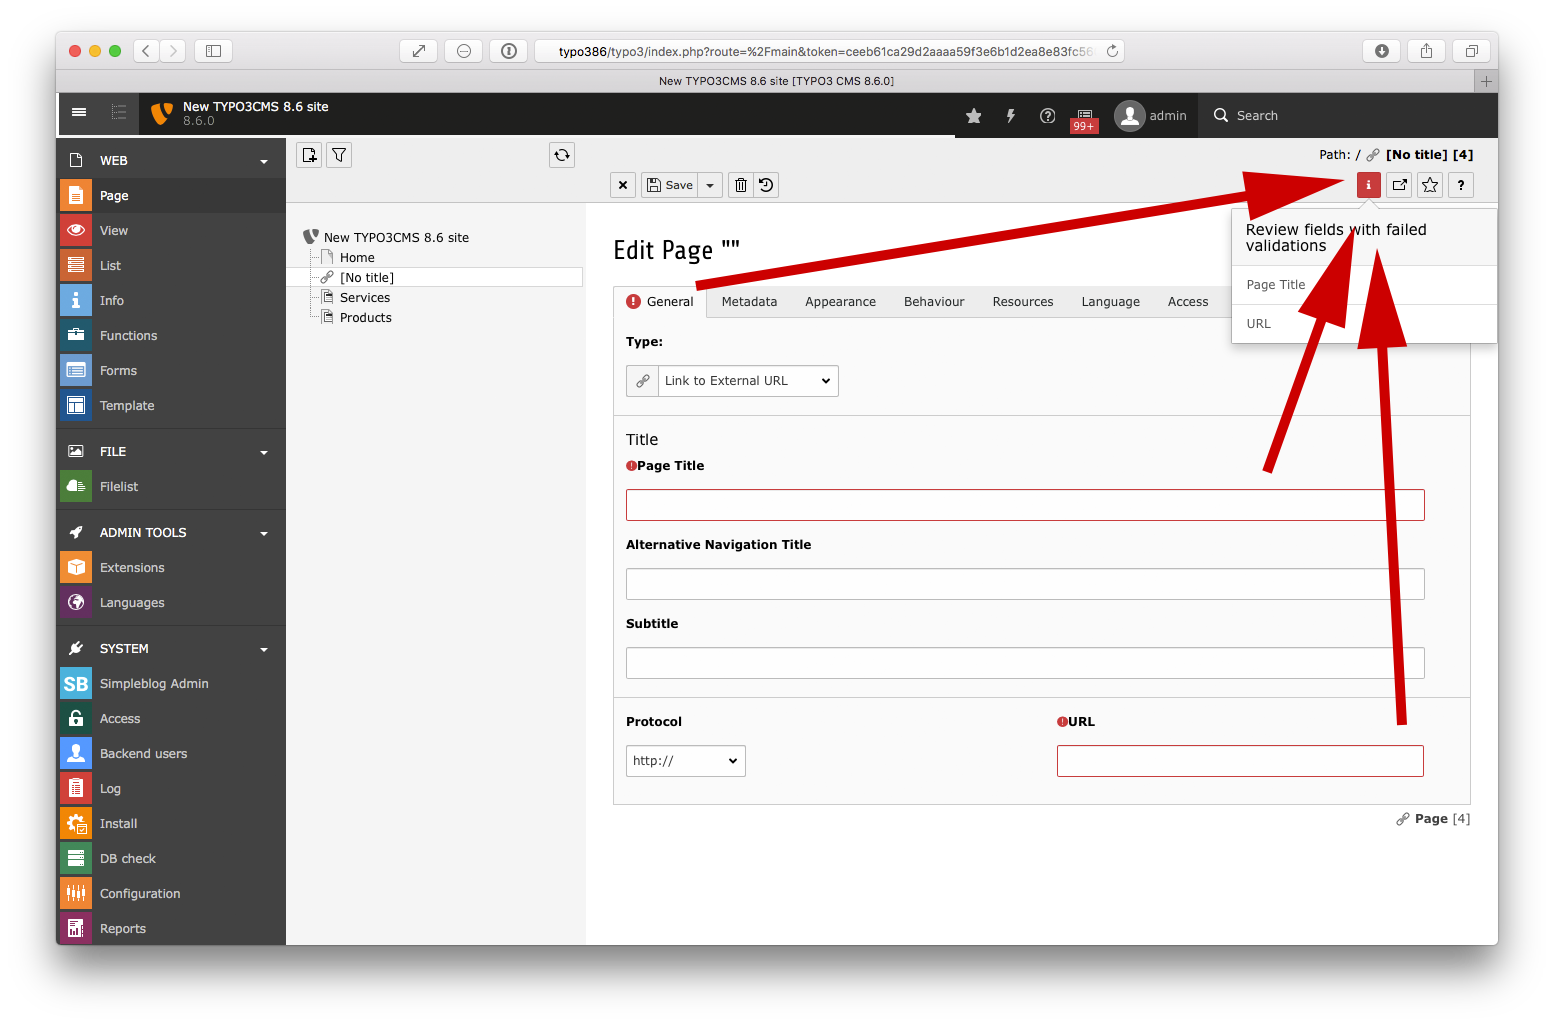
\includegraphics[width=0.99\linewidth]{BackendUserInterface/79521.png}
			\end{figure}
		\end{column}
	\end{columns}

\end{frame}

% ------------------------------------------------------------------------------
% LTXE-SLIDE-START
% LTXE-SLIDE-UID:		1d2c526e-290be77d-f92d1039-0b74486e
% LTXE-SLIDE-ORIGIN:	749a055b-02003192-92f2631e-39abcc95 English
% LTXE-SLIDE-TITLE:		#79622: Dedicated content elements for menus
% LTXE-SLIDE-REFERENCE:	!Breaking: #79622 - Dedicated content elements for menus
% ------------------------------------------------------------------------------
\begin{frame}[fragile]
	\frametitle{Gebruikersinterface backend}
	\framesubtitle{Aparte inhoudselementen voor menu's}

	Om het onderhoud te verbeteren is het huidige inhoudselement menu opgedeeld in
	aparte inhoudselementen.

	\begin{figure}\vspace{-0.2cm}
		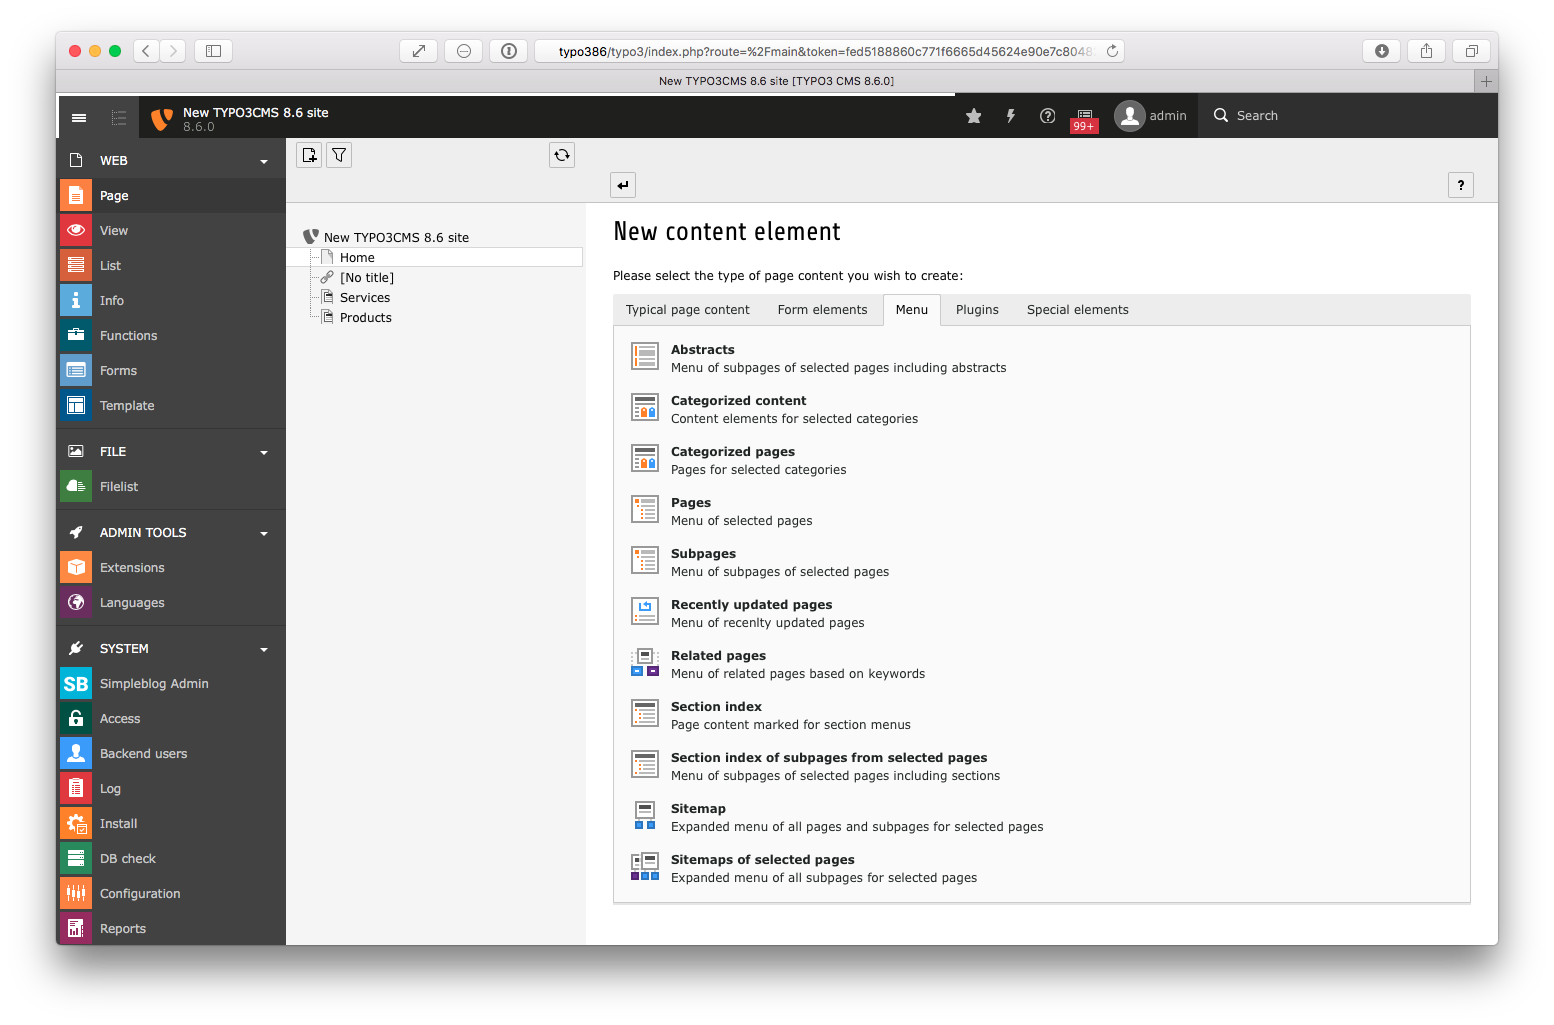
\includegraphics[width=0.68\linewidth]{BackendUserInterface/79622.png}
	\end{figure}

\end{frame}

% ------------------------------------------------------------------------------
